% ==================================================
% 2. USE-CASE SPECIFICATIONS
% ==================================================
\section{Use-case Specifications}
This section describes the use cases of the
Medication Safety Assistant research prototype.
Each use case represents a user goal and an
observable result.
The use cases are organized by common user
workflows and supporting roles. Their order
does not imply a required execution sequence.
HCP reviews are simulated, and future
features are excluded.

% UC-01 to UC-05 - updated against Use-Case Specification v1.0 (1 Nov 2026)
% Required packages in the MAIN document preamble:
% \usepackage{xcolor}
% \usepackage{graphicx}
% \usepackage{float}
% \usepackage{longtable}
% Changes relative to the old specification are highlighted in blue.
% New diagram captions are blue; the supplied diagram image content is preserved.
% Place UC-01.png ... UC-05.png in an images/ folder beside the main .tex file.
\providecommand{\UCchange}[1]{\textcolor{blue}{#1}}
% ==================== UC-01 ====================
\subsection{Use-case: Sign In}
\label{uc:uc-01}
\begin{figure}[H]
\centering
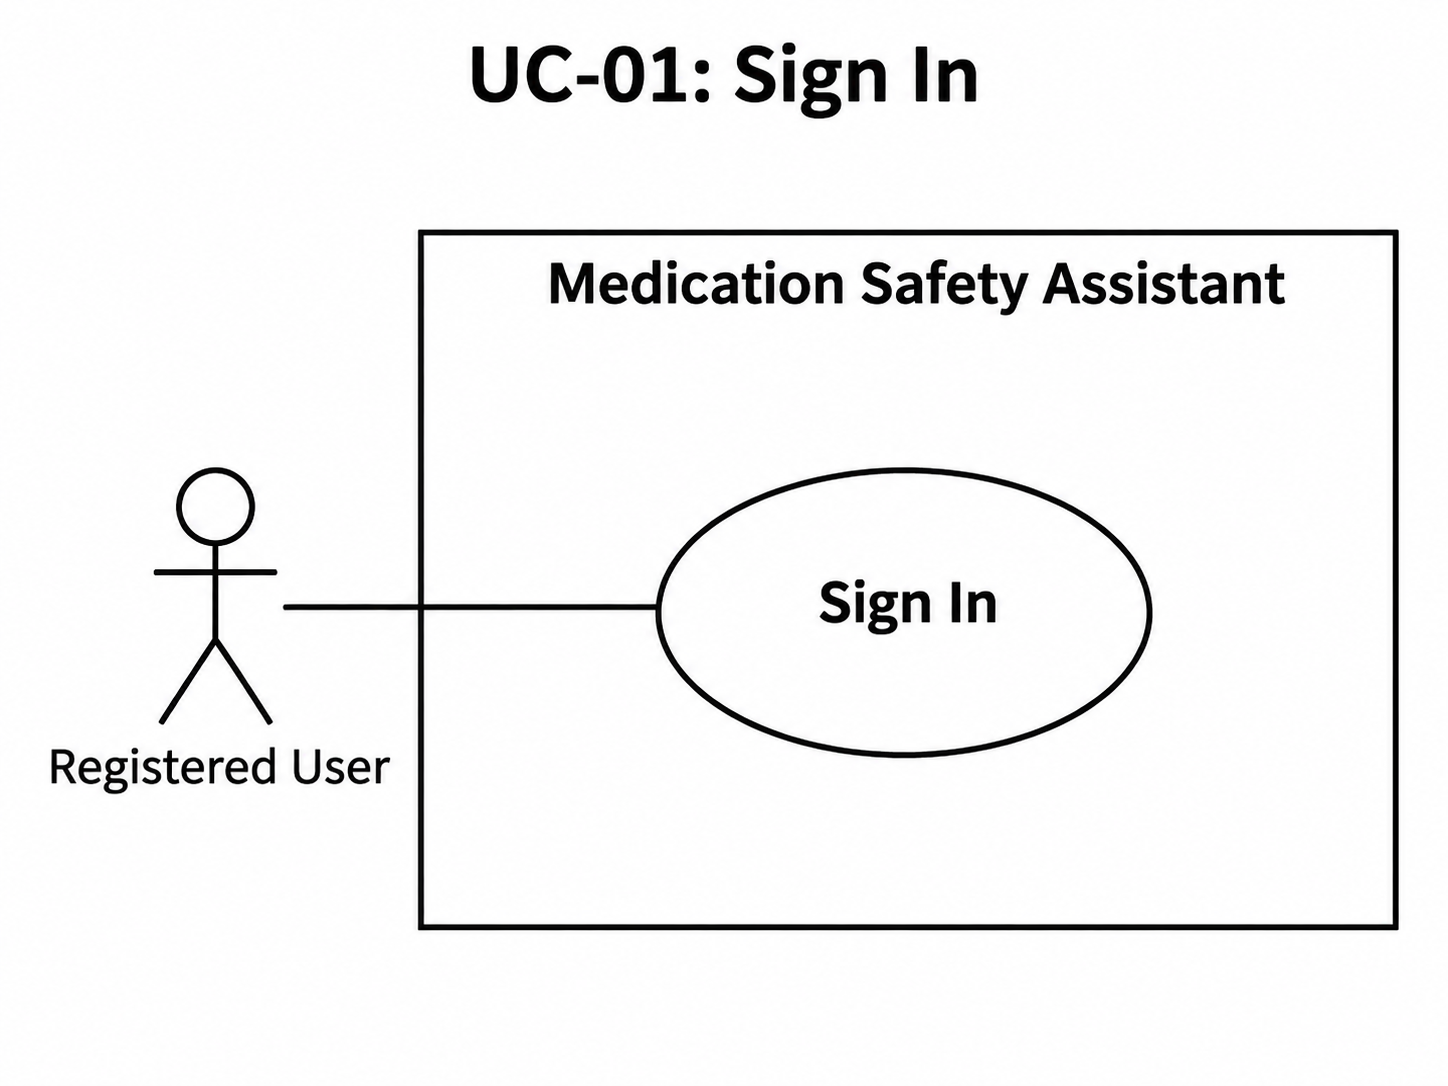
\includegraphics[width=0.91\textwidth,height=0.245\textheight,keepaspectratio]{images/UC-01.png}
\caption{\UCchange{UC-01: Detailed use-case model.}}
\label{fig:uc-01}
\end{figure}
\begin{longtable}{|p{0.20\textwidth}|p{0.70\textwidth}|}
\hline
\textbf{Use case Name} & UC-01: Sign In \\ \hline
\textbf{Brief description} & A registered user signs in and receives access to the features permitted by their role. \\ \hline
\textbf{Actors} & Patient / General User; Healthcare Professional (HCP); Dataset Reviewer; Administrator; Technical Support \\ \hline
\textbf{Basic Flow} &
1. The user enters an account name and password.\par
2. The system checks the credentials and account status.\par
3. The system verifies the assigned role and permissions.\par
4. The system creates an authenticated session and opens the permitted dashboard.\par
\\ \hline
\textbf{Alternative Flows} &
\UCchange{\textbf{A1. Incorrect credentials (step 2)}}\par
\UCchange{The system shows an error without creating a session. The user may retry or cancel.}\par
\par\smallskip
\UCchange{\textbf{A2. Inactive or blocked account (step 2)}}\par
\UCchange{The system denies access. No session is created.}\par
\par\smallskip
\UCchange{\textbf{A3. Role permissions are unavailable (step 3)}}\par
\UCchange{The system denies access rather than creating an unrestricted session.}\par
\\ \hline
\textbf{Pre-conditions} & The user has a registered account and can open the sign-in page. \\ \hline
\textbf{Post-conditions} &
\textbf{Success:} \UCchange{A session is created with verified role permissions.}\par
\textbf{Failure:} No authenticated session is created. \\ \hline
\end{longtable}
% ==================== UC-02 ====================
\subsection{Use-case: Enter and Confirm Medication Information}
\label{uc:uc-02}
\begin{figure}[H]
\centering
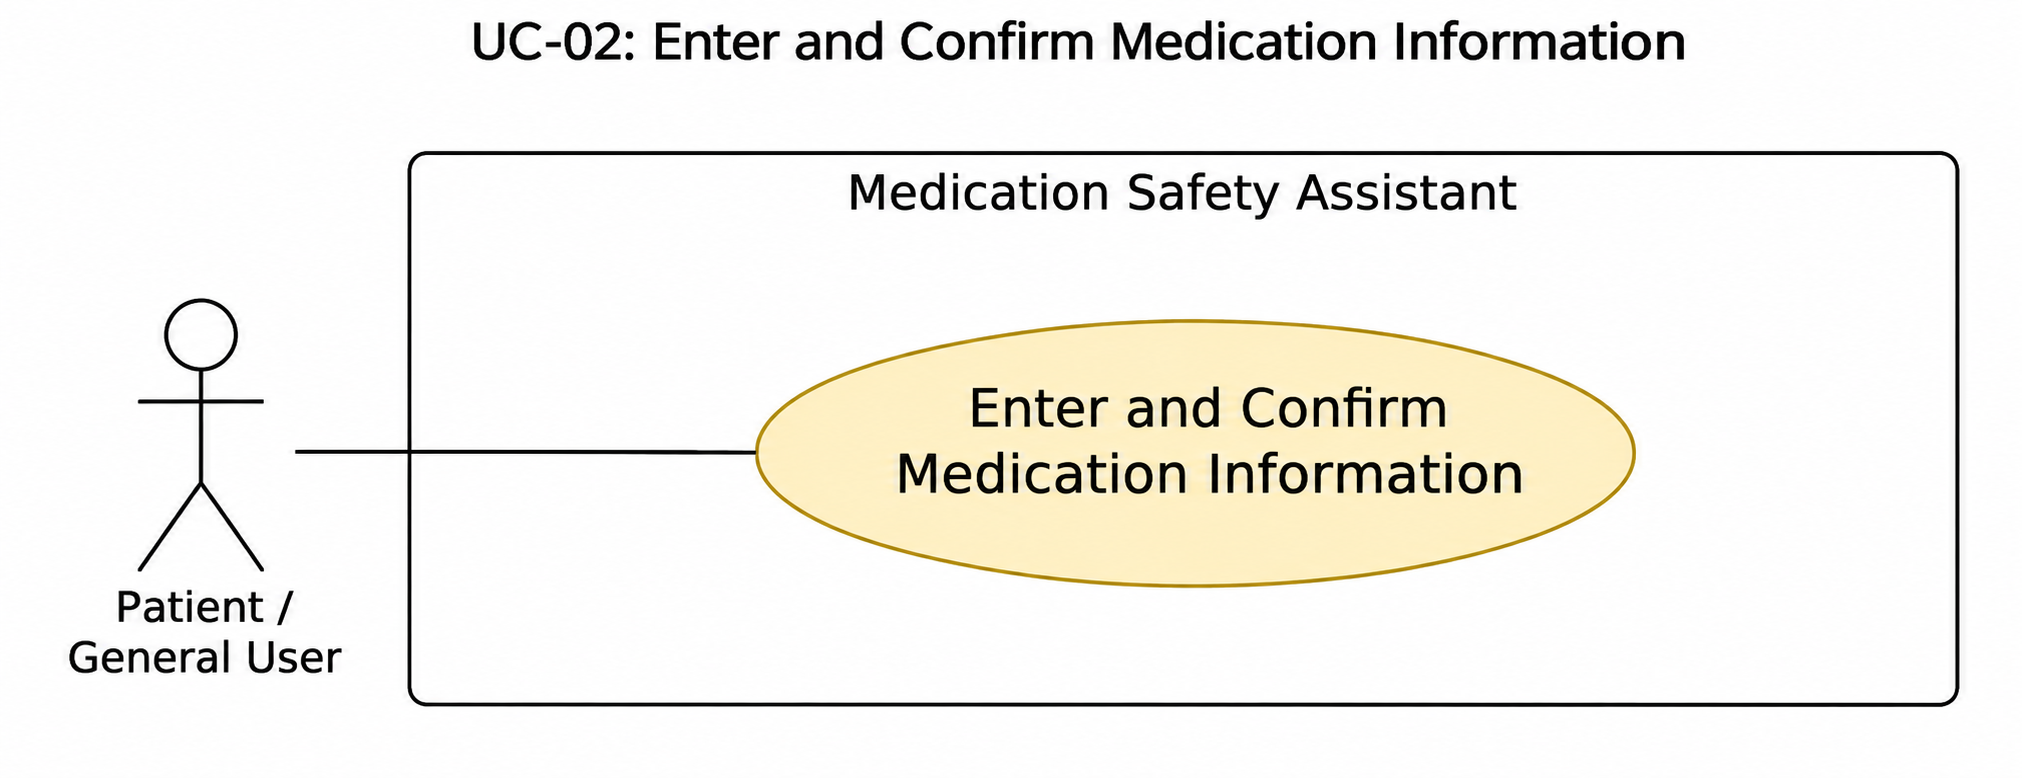
\includegraphics[width=0.91\textwidth,height=0.245\textheight,keepaspectratio]{images/UC-02.png}
\caption{\UCchange{UC-02: Detailed use-case model.}}
\label{fig:uc-02}
\end{figure}
\begin{longtable}{|p{0.20\textwidth}|p{0.70\textwidth}|}
\hline
\textbf{Use case Name} & UC-02: Enter and Confirm Medication Information \\ \hline
\textbf{Brief description} & The patient enters medication information through a supported method and confirms the recorded details before further use. \\ \hline
\textbf{Actors} & Patient / General User \\ \hline
\textbf{Basic Flow} &
\UCchange{1. The patient provides medication details by manual entry, OCR image, or chatbot text.}\par
\UCchange{2. The system processes the input and clarifies the intended task when needed.}\par
\UCchange{3. The system displays the recorded details and marks any missing or uncertain fields.}\par
\UCchange{4. The patient corrects errors and explicitly confirms that the details match the source.}\par
\UCchange{5. The system saves the confirmed entries and any remaining information gaps.}\par
\\ \hline
\textbf{Alternative Flows} &
\UCchange{\textbf{A1. Input is unclear or incomplete (steps 2--3)}}\par
\UCchange{The system asks for missing details or marks unresolved fields. The patient may correct them before confirming.}\par
\par\smallskip
\UCchange{\textbf{A2. Input processing fails (step 2)}}\par
\UCchange{The system offers a retry or another supported input method. No unconfirmed entry is released.}\par
\par\smallskip
\UCchange{\textbf{A3. Patient does not confirm (step 4)}}\par
\UCchange{The input remains unconfirmed and cannot be used for safety assessment or reminder activation.}\par
\\ \hline
\textbf{Pre-conditions} & The patient is signed in and can access medication entry. \\ \hline
\textbf{Post-conditions} &
\textbf{Success:} \UCchange{Confirmed input is saved for later identification and supported checks; confirmation does not prove medicine identity or safety.}\par
\textbf{Failure:} Unconfirmed input is not used for safety checks or reminder activation. \\ \hline
\end{longtable}
% ==================== UC-03 ====================
\subsection{Use-case: Check Medication Safety}
\label{uc:uc-03}
\begin{figure}[H]
    \centering
    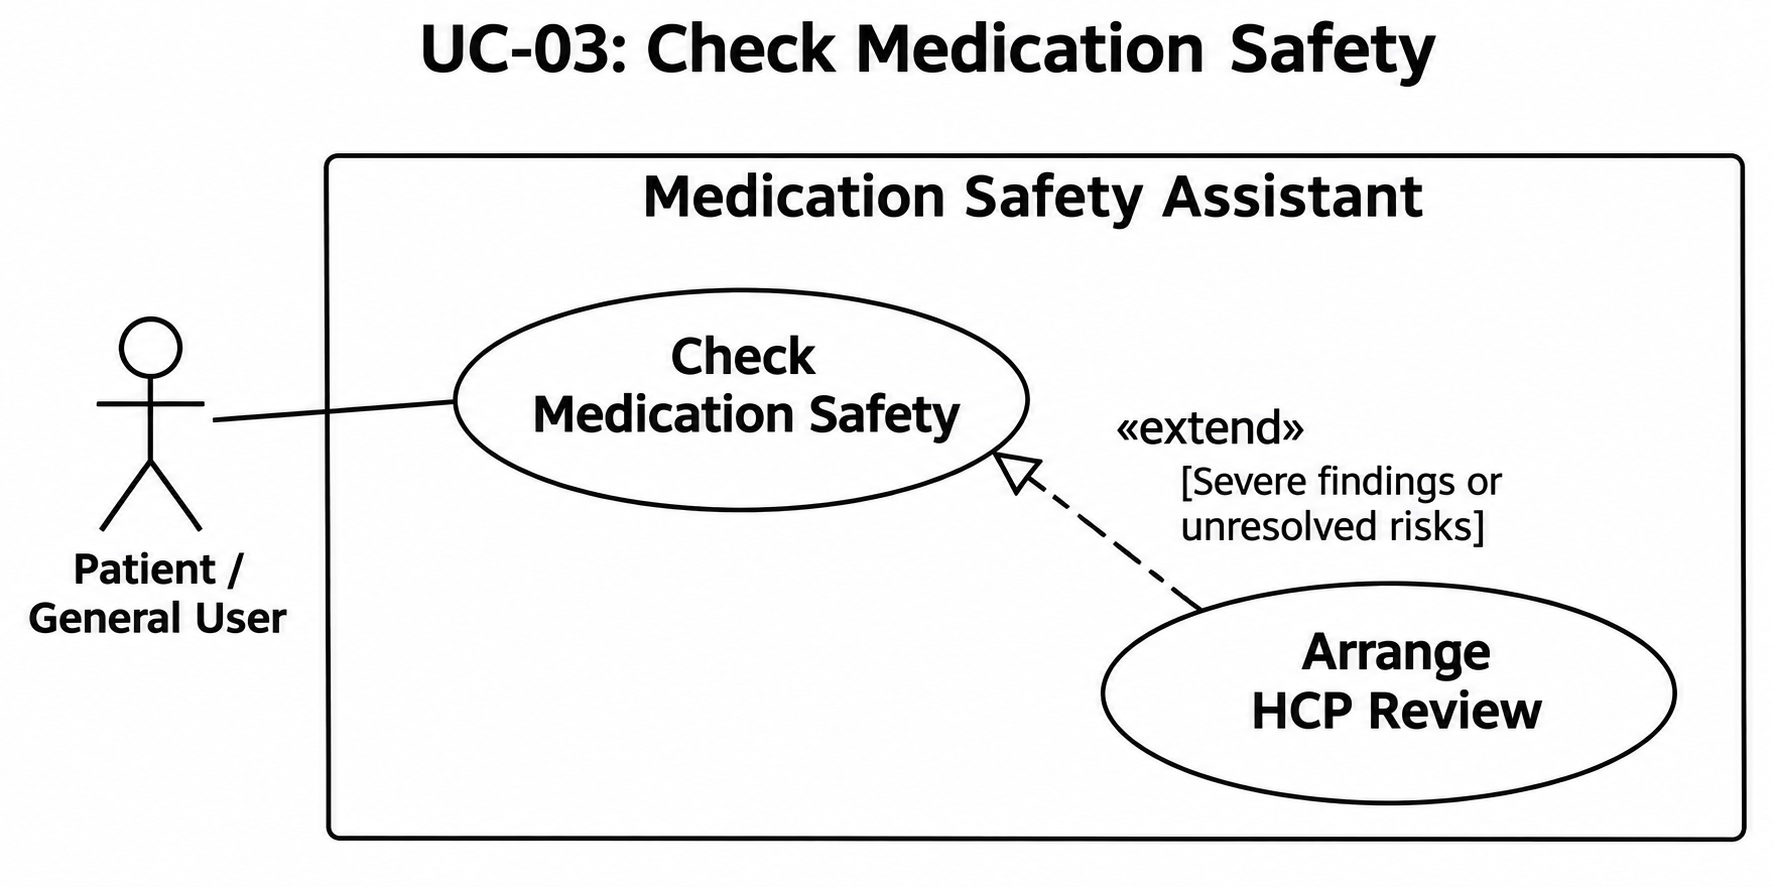
\includegraphics[width=0.91\textwidth,height=0.245\textheight,keepaspectratio]{images/UC-03.png}
    \caption{UC-03: Detailed use-case model.}
    \label{fig:uc-03}
\end{figure}
\begin{longtable}{|p{0.20\textwidth}|p{0.70\textwidth}|}
\hline
\textbf{Use case Name} & UC-03: Check Medication Safety \\ \hline
\textbf{Brief description} &
The patient receives supported medication risk findings, warnings, data limitations, and next steps without automatic treatment changes. \\ \hline
\textbf{Actors} & Patient / General User \\ \hline
\textbf{Basic Flow} &
1. The patient requests a safety check using confirmed medication information.\par
2. The system identifies assessable medicines and active ingredients using supported reference data.\par
\UCchange{3. The system retrieves available medical conditions and allergies from the patient's health profile (UC-18), including their information sources.}\par
\UCchange{4. The system performs supported checks for drug--drug interactions, duplicate ingredients, drug--disease risks, and applicable contraindication or allergy risks.}\par
5. The system records findings, risk levels, unassessed checks, and data limitations.\par
6. The system saves the assessment, its status, and its time.\par
7. The system shows warnings and next steps, and offers UC-04 when severe or unresolved risks need HCP review.
\\ \hline
\textbf{Alternative Flows} &
\textbf{A1. Medicine or reference data is unavailable (steps 2--4)}\par
The system marks affected checks as Unassessed, performs other supported checks where possible, and does not claim the medicine is safe.\par\smallskip
\UCchange{\textbf{A2. Health profile information is missing or uncertain (steps 3--4)}}\par
\UCchange{The system marks affected patient-specific checks as Unassessed or limited and continues independent supported checks. Missing information is not treated as the absence of risk.}\par\smallskip
\textbf{A3. Severe drug--drug interaction is found (step 4)}\par
The system records a severe warning and holds affected new reminders pending HCP review. Existing reminders and treatment remain unchanged.\par\smallskip
\textbf{A4. Assessment fails (steps 2--6)}\par
The system reports an incomplete or failed check and retains previously recorded warnings and reminder restrictions.
\\ \hline
\textbf{Pre-conditions} &
The patient is signed in and has at least one confirmed medication record. \\ \hline
\textbf{Post-conditions} &
\textbf{Success:} A saved assessment shows supported findings and limitations. Affected new reminders remain on hold when required by the safety rules until a recorded HCP review and recheck permit them.\par
\textbf{Failure:} No incomplete or failed check is presented as safe; treatment and existing reminders remain unchanged.
\\ \hline
\end{longtable}
% ==================== UC-04 ====================
\subsection{Use-case: Arrange HCP Review}
\label{uc:uc-04}
\begin{figure}[H]
    \centering
    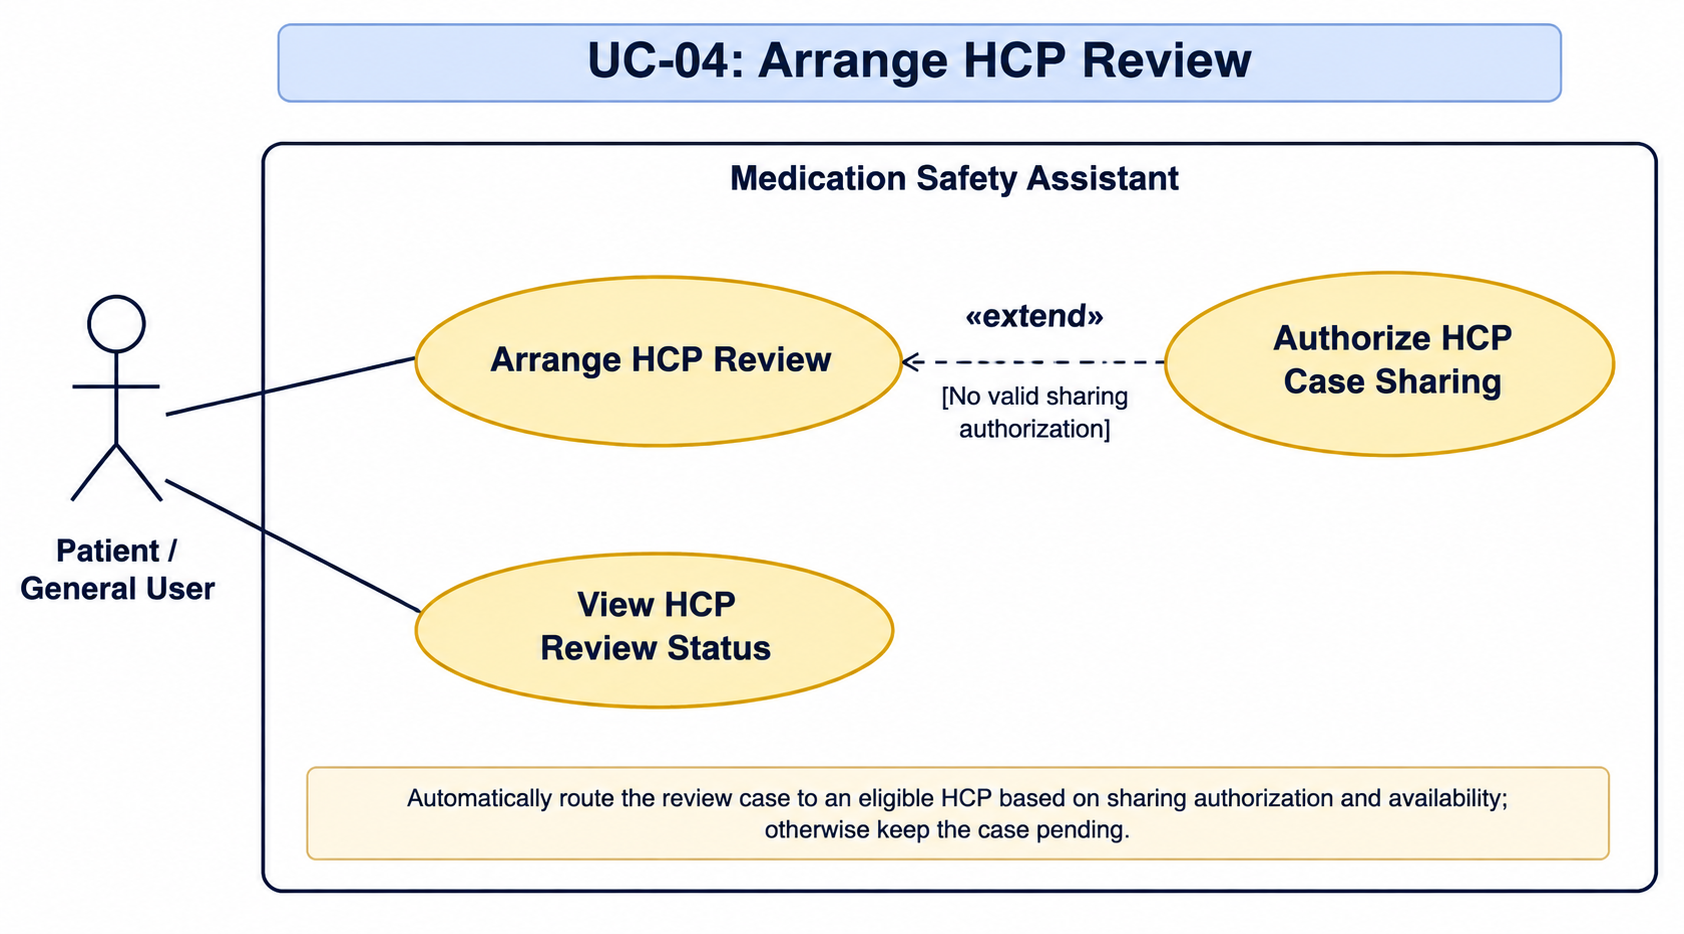
\includegraphics[width=0.91\textwidth,height=0.245\textheight,keepaspectratio]{images/UC-04.png}
    \caption{UC-04: Detailed use-case model.}
    \label{fig:uc-04}
\end{figure}
\begin{longtable}{|p{0.20\textwidth}|p{0.70\textwidth}|}
\hline
\textbf{Use case Name} & UC-04: Arrange HCP Review \\ \hline
\textbf{Brief description} &
\UCchange{The patient arranges a simulated HCP review for a saved safety assessment or a pending medication schedule request, with case-specific sharing permission and authorized assignment.} \\ \hline
\textbf{Actors} & Patient / General User \\ \hline
\textbf{Basic Flow} &
\UCchange{1. The patient selects a saved safety assessment (UC-03) or a pending schedule verification or change request (UC-06/UC-07).}\par
\UCchange{2. The system shows the review purpose, relevant warnings or schedule details, missing information, and proposed sharing scope.}\par
3. The system reuses an active request or creates a pending request without granting HCP access.\par
4. The patient reviews and authorizes case-specific sharing if valid permission is not already available.\par
5. The system validates the permission and assigns an eligible, available HCP when possible.\par
6. The system displays the review request status to the patient.
\\ \hline
\textbf{Alternative Flows} &
\textbf{A1. Sharing is not authorized (step 4)}\par
The request waits for permission. No HCP receives access, and no review starts.\par\smallskip
\textbf{A2. No eligible HCP is available (step 5)}\par
The request remains Pending Assignment and is not reported as reviewed.\par\smallskip
\textbf{A3. An active request already exists (step 3)}\par
The system reuses the existing request instead of creating a duplicate.\par\smallskip
\textbf{A4. Request or assignment cannot be saved (steps 3 or 5)}\par
The system reports the error and grants no new access or assignment.
\\ \hline
\textbf{Pre-conditions} &
\UCchange{The patient is signed in and has a saved safety assessment or a saved pending schedule request. HCP access requires valid case-sharing permission.} \\ \hline
\textbf{Post-conditions} &
\textbf{Success:} The request is waiting for authorization, pending assignment, or assigned to an authorized HCP; the patient can view its status.\par
\textbf{Failure:} No unauthorized access or duplicate request is created. Existing warnings, reminder restrictions, and verified schedules remain unchanged.
\\ \hline
\end{longtable}
% ==================== UC-05 ====================
\subsection{Use-case: Review Medication Safety Case}
\label{uc:uc-05}
\begin{figure}[H]
    \centering
    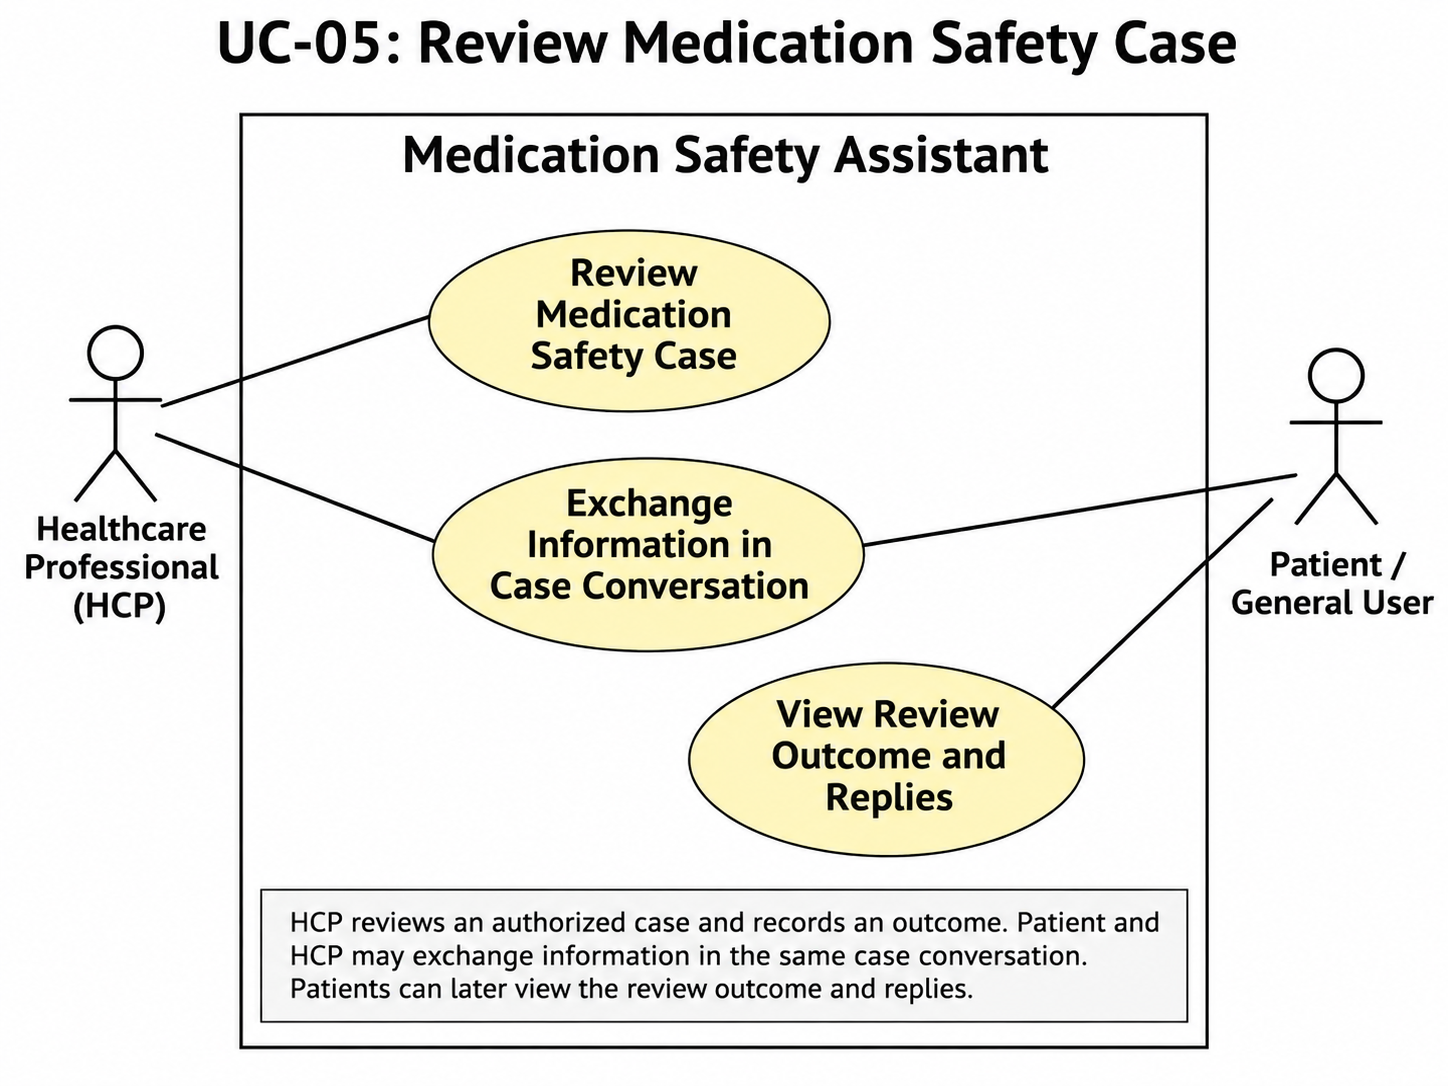
\includegraphics[width=0.91\textwidth,height=0.245\textheight,keepaspectratio]{images/UC-05.png}
    \caption{UC-05: Detailed use-case model.}
    \label{fig:uc-05}
\end{figure}
\begin{longtable}{|p{0.20\textwidth}|p{0.70\textwidth}|}
\hline
\textbf{Use case Name} & UC-05: Review Medication Safety Case \\ \hline
\textbf{Brief description} &
\UCchange{An authorized HCP reviews a shared medication safety case or related schedule request, exchanges information with the patient, and records a simulated review outcome.} \\ \hline
\textbf{Actors} & Healthcare Professional (HCP); Patient / General User \\ \hline
\textbf{Basic Flow} &
1. The HCP opens an assigned review request with valid patient sharing permission.\par
\UCchange{2. The system shows the permitted safety findings or proposed schedule, existing instructions and their sources, and the case conversation.}\par
\UCchange{3. The HCP reviews the evidence and records a relevant outcome, comments, or a request for more information.}\par
4. The system saves the outcome, responsible HCP, time, and related replies.\par
\UCchange{5. If the outcome confirms a schedule or resolves a required review, the system rechecks affected pending new reminders against the remaining verification and safety rules. It does not change treatment or activate an ineligible reminder.}\par
6. The patient can view the recorded outcome and replies.
\\ \hline
\textbf{Alternative Flows} &
\textbf{A1. More information is needed (step 3)}\par
The HCP requests details in the same case conversation. The patient may reply, and the case returns to the HCP queue. No unrecorded approval is assumed.\par\smallskip
\textbf{A2. Patient sends a follow-up (after step 6)}\par
The system records the reply in the same permitted thread and returns the case for further review when appropriate.\par\smallskip
\textbf{A3. Case remains unresolved (step 3)}\par
The HCP records the reason. Required safety warnings and new-reminder holds remain in place.\par\smallskip
\UCchange{\textbf{A4. Proposed schedule is not confirmed (step 3)}}\par
\UCchange{The HCP records the outcome. The proposed timing is not applied, and the current verified schedule remains unchanged.}\par\smallskip
\textbf{A5. Access is invalid or saving fails (steps 1 or 4)}\par
The system blocks the action or reports failure. No unrecorded outcome is treated as approval.
\\ \hline
\textbf{Pre-conditions} &
The HCP is signed in, assigned to the review request, and authorized by the patient to access the shared details. \\ \hline
\textbf{Post-conditions} &
\textbf{Success:} A traceable simulated review outcome or conversation update is saved and visible to permitted participants. Any new-reminder change is subject to a separate safety recheck.\par
\textbf{Failure:} No unauthorized data is disclosed, and no treatment or reminder restriction is changed by an unrecorded decision.
\\ \hline
\end{longtable}
% ==================== UC-06 ====================
\subsection{Use-case: Set Up Medication Reminders}
\label{uc:uc-06}
\InlineUCModel{06}
\begin{longtable}{|p{0.20\textwidth}|p{0.71\textwidth}|}
\hline
\textbf{Use case Name} & UC-06: Set Up Medication Reminders \\ \hline
\textbf{Brief description} &
The patient activates reminders from an existing verified prescription or recorded HCP schedule when the applicable safety rules allow it. \\ \hline
\textbf{Actors} & Patient / General User \\ \hline
\textbf{Basic Flow} &
\UCchange{1. The patient selects a saved medication for reminder setup.}\par
2. The system displays the recorded schedule, its source, and relevant safety status.\par
3. The patient confirms that the schedule matches the existing instructions.\par
4. The system checks schedule verification, recorded risk warnings, and the new-reminder safety gate.\par
5. The system activates eligible reminders and shows their status.
\\ \hline
\textbf{Alternative Flows} &
\textbf{A1. Schedule is missing or unverified (steps 2--4)}\par
The system does not activate reminders. The patient may correct or supply existing instructions; a saved verification request may be submitted for HCP review through UC-04.\par\smallskip
\textbf{A2. Patient proposes new timing (step 3)}\par
The system saves the proposal as Pending HCP Review and offers UC-04. The proposed schedule is not activated without recorded HCP confirmation and a safety recheck.\par\smallskip
\textbf{A3. Severe interaction affects the medicine (step 4)}\par
Affected new reminders remain on hold, and the system offers UC-04. Other eligible reminders may activate; existing reminders and treatment are not stopped automatically.\par\smallskip
\textbf{A4. Safety check is unavailable (step 4)}\par
The system reports Unassessed rather than safe clearance. Affected new reminders remain restricted when the applicable rules require review.\par\smallskip
\textbf{A5. Browser notifications are unavailable (step 5)}\par
The system reports the limitation. Eligible schedules remain visible in the application without claiming browser notifications are enabled.
\\ \hline
\textbf{Pre-conditions} &
The patient is signed in and has a saved medication record for which reminder setup can be requested. \\ \hline
\textbf{Post-conditions} &
\textbf{Success:} An eligible reminder setting is saved, or a pending verification or timing request is recorded for review.\par
\textbf{Failure:} No unconfirmed or failed schedule change is applied. Any previous reminder settings remain unchanged.
\\ \hline
\end{longtable}
% ==================== UC-07 ====================
\subsection{Use-case: Manage Medication Reminders}
\label{uc:uc-07}
\InlineUCModel{07}
\begin{longtable}{|p{0.20\textwidth}|p{0.71\textwidth}|}
\hline
\textbf{Use case Name} & UC-07: Manage Medication Reminders \\ \hline
\textbf{Brief description} &
The patient manages permitted notification settings or proposes reminder timing changes without changing prescribed treatment. \\ \hline
\textbf{Actors} & Patient / General User \\ \hline
\textbf{Basic Flow} &
1. The patient opens an existing reminder and chooses to manage it.\par
2. The system shows the current schedule, its source, and notification settings.\par
3. The patient requests a notification change or a schedule update.\par
4. The system checks the requested change against verified instructions and applicable safety rules.\par
5. The patient confirms the request.\par
\UCchange{6. The system saves an allowed notification or schedule setting, or stores a timing proposal as Pending HCP Review without applying it.}
\\ \hline
\textbf{Alternative Flows} &
\textbf{A1. Patient disables notifications (step 3)}\par
The system prepares to disable only the selected notification. After patient confirmation, it saves the change. The verified medication schedule remains unchanged.\par\smallskip
\textbf{A2. Timing differs from verified instructions (step 4)}\par
The system marks the timing proposal as requiring HCP review and offers UC-04. The previous verified schedule remains effective unless the proposal is confirmed and passes a new safety check.\par\smallskip
\textbf{A3. Patient cancels or update fails (steps 5--6)}\par
The system keeps the previous reminder settings and reports a save error when relevant.
\\ \hline
\textbf{Pre-conditions} &
The patient is signed in and owns an existing reminder. \\ \hline
\textbf{Post-conditions} &
\textbf{Success:} A permitted setting is saved, a notification is disabled as requested, or a timing proposal is recorded as Pending HCP Review.\par
\UCchange{\textbf{Failure:} Previous reminder settings remain unchanged.}
\\ \hline
\end{longtable}
% UC-08 - Record Dose Status | from UC-09
\subsection{Use-case: Record Dose Status}
\label{uc:uc-08}
\InlineUCModel{08}
\begin{longtable}{|p{0.20\textwidth}|p{0.71\textwidth}|}
\hline
\textbf{Use case Name} & UC-08: Record Dose Status \\ \hline
\textbf{Brief description} & The patient records whether a scheduled medication dose was Taken, Missed, or Skipped for adherence tracking. \\ \hline
\textbf{Actors} & Patient / General User \\ \hline
\textbf{Basic Flow} &
1. The patient selects a scheduled dose from the reminder or adherence view.\par
2. The system shows the medicine, scheduled time, and current dose status.\par
3. The patient selects Taken, Missed, or Skipped.\par
4. The patient confirms the entry.\par
5. The system saves the dose status and recorded time.
\\ \hline
\textbf{Alternative Flows} &
\textbf{A1. Existing entry is corrected (step 3)}\par
1. The system shows the previous status for comparison.\par
2. The patient confirms the correction; continue to step 5.
\par\smallskip
\textbf{A2. Patient cancels (step 4)}\par
1. The system keeps the previous entry and ends the use case.
\par\smallskip
\textbf{A3. Dose event is unavailable or save fails (steps 2 or 5)}\par
1. The system explains that the entry cannot be saved.\par
2. No unsupported dose record is created.
\\ \hline
\textbf{Pre-conditions} & The patient is signed in and has an accessible scheduled dose or adherence entry. \\ \hline
\textbf{Post-conditions} & \textbf{Success:} The confirmed dose status is saved and available in adherence history.\par
\textbf{Failure:} No dose entry is changed; no treatment recommendation is produced. \\ \hline
\end{longtable}
% UC-09 - View Adherence History | from UC-10
\subsection{Use-case: View Adherence History}
\label{uc:uc-09}
\InlineUCModel{09}
\begin{longtable}{|p{0.20\textwidth}|p{0.71\textwidth}|}
\hline
\textbf{Use case Name} & UC-09: View Adherence History \\ \hline
\textbf{Brief description} & The patient reviews recorded medication use over time. \\ \hline
\textbf{Actors} & Patient / General User \\ \hline
\textbf{Basic Flow} &
1. The patient opens Adherence History.\par
2. The system shows available scheduled doses and recorded statuses.\par
3. The patient may select a medicine
or time period to filter the history.\par
4. The system displays the available
records matching the selected filter,
or all permitted records if no
filter is selected.
\\ \hline
\textbf{Alternative Flows} &
\textbf{A1. No entries match (step 4)}\par
1. The system shows an empty result and allows another filter.
\par\smallskip
\textbf{A2. History is incomplete or unavailable (step 2)}\par
1. The system displays available records and reports any unavailable period.
\\ \hline
\textbf{Pre-conditions} & The patient is signed in and can view their own adherence records. \\ \hline
\textbf{Post-conditions} & \textbf{Success:} Permitted adherence history is displayed without modifying it.\par
\textbf{Failure:} No record is changed. \\ \hline
\end{longtable}
% ---------- 05. Records and history ----------
% UC-10 - View Medication and Safety History | from UC-06
\subsection{Use-case: View Medication and Safety History}
\label{uc:uc-10}
\InlineUCModel{10}
\begin{longtable}{|p{0.20\textwidth}|p{0.71\textwidth}|}
\hline
\textbf{Use case Name} & UC-10: View Medication and Safety History \\ \hline
\textbf{Brief description} & The patient reviews saved medication records, past safety results, review outcomes, and their dates. \\ \hline
\textbf{Actors} & Patient / General User \\ \hline
\textbf{Basic Flow} &
1. The patient opens Medication and Safety History.\par
2. The system lists permitted medication records and past safety assessments.\par
3. The patient selects a record or assessment.\par
4. The system shows its date, findings, limitations, and linked HCP review status.\par
5. The system clearly labels results that no longer match the current medication record.
\\ \hline
\textbf{Alternative Flows} &
\textbf{A1. No history is available (step 2)}\par
1. The system displays an empty-state message and ends the use case.
\par\smallskip
\textbf{A2. A record is no longer available or access is denied (step 3)}\par
1. The system reports the limitation without showing private data.\par
2. The patient may select another permitted record.
\\ \hline
\textbf{Pre-conditions} & The patient is signed in and can view their own records. \\ \hline
\textbf{Post-conditions} & \textbf{Success:} Historical information is displayed without changing stored data.\par
\textbf{Failure:} No record or treatment is changed. \\ \hline
\end{longtable}
% ============================================================
% 06. CHATBOT AND PATIENT HEALTH SUMMARY
% ============================================================
% UC-11 - Ask a Medication Question
\clearpage
\subsection{Use-case: Ask a Medication Question}
\label{uc:uc-11}
\InlineUCModel{11}
\begin{longtable}{|p{0.20\textwidth}|p{0.71\textwidth}|}
\hline
\endfirsthead
\multicolumn{2}{l}{\textbf{UC-11: Specification (continued)}}\\\\
\hline
\endhead
\textbf{Use case Name} & UC-11: Ask a Medication Question \\ \hline
\textbf{Brief description} &
The patient receives a supported medication-related answer from the chatbot with appropriate limits.
\\ \hline
\textbf{Actors} & Patient / General User \\ \hline
\textbf{Basic Flow} &
\textcolor{blue}{1. The patient enters a medication-related question in the chatbot.}\par
\textcolor{blue}{2. The system identifies the question and retrieves relevant approved reference information and permitted patient context.}\par
\textcolor{blue}{3. The system prepares an answer with supporting information and relevant limitations.}\par
\textcolor{blue}{4. The system displays the answer or asks a follow-up question when clarification is needed.}\par
\textcolor{blue}{5. The patient may open View Conversation History to review previous conversations.}
\\ \hline
\textbf{Alternative Flows} &
\textcolor{blue}{\textbf{A1. Question is unclear (step 2)}}\par
\textcolor{blue}{1. The system asks a short follow-up question.}\par
\textcolor{blue}{2. If clarified, return to step 2; otherwise, end the use case.}
\\ \hline
\textbf{Alternative Flows} &
\textcolor{blue}{\textbf{A2. Patient requests source details (step 3)}}\par
\textcolor{blue}{1. The system displays the available supporting sources through View Supporting References.}\par
\textcolor{blue}{2. The patient may return to the answer.}
\\ \hline
\textbf{Alternative Flows} &
\textcolor{blue}{\textbf{A3. Reliable information is unavailable (step 3)}}\par
\textcolor{blue}{1. The system explains the information limit instead of generating unsupported medical claims.}
\\ \hline
\textbf{Alternative Flows} &
\textcolor{blue}{\textbf{A4. Request requires a clinical decision or another workflow (step 2)}}\par
\textcolor{blue}{1. The chatbot does not diagnose, prescribe, or change treatment.}\par
\textcolor{blue}{2. The system directs the patient to the appropriate supported workflow or qualified HCP when necessary.}\par
\textcolor{blue}{3. No medication record is changed solely from an unconfirmed chatbot message.}
\\ \hline
\textbf{Pre-conditions} & The patient is signed in and the chatbot is available. \\ \hline
\textbf{Post-conditions} & \textbf{Success:} The patient receives a supported answer, clarification, or clear limitation.\par
\textbf{Failure:} No unsupported clinical decision or unconfirmed record change occurs. \\ \hline
\end{longtable}
% UC-12 - Generate Patient Health Summary
\clearpage
\subsection{Use-case: Generate Patient Health Summary}
\label{uc:uc-12}
\InlineUCModel{12}
\begin{longtable}{|p{0.20\textwidth}|p{0.71\textwidth}|}
\hline
\endfirsthead
\multicolumn{2}{l}{\textbf{UC-12: Specification (continued)}}\\\\
\hline
\endhead
\textbf{Use case Name} & UC-12: Generate Patient Health Summary \\ \hline
\textbf{Brief description} &
\textcolor{blue}{The patient generates a structured summary from confirmed medication records and patient health information for review and optional sharing.}
\\ \hline
\textbf{Actors} & Patient / General User \\ \hline
\textbf{Basic Flow} &
\textcolor{blue}{1. The patient requests a Patient Health Summary.}\par
\textcolor{blue}{2. The system retrieves confirmed medication records, health conditions, allergies, and available safety assessment results.}\par
\textcolor{blue}{3. The system prepares a draft summary with information sources, dates, medication status, and known information gaps.}\par
\textcolor{blue}{4. The patient reviews the draft through Review and Confirm Draft Summary and corrects inaccurate information when necessary.}\par
\textcolor{blue}{5. The patient confirms the summary, and the system saves it for later viewing or optional sharing.}
\\ \hline
\textbf{Alternative Flows} &
\textcolor{blue}{\textbf{A1. Confirmed information is incomplete (step 2)}}\par
\textcolor{blue}{1. The system identifies missing information and prepares a limited draft using available confirmed data.}\par
\textcolor{blue}{2. If no eligible information is available, the system asks the patient to provide or confirm the required information.}
\\ \hline
\textbf{Alternative Flows} &
\textcolor{blue}{\textbf{A2. The draft needs correction (step 4)}}\par
\textcolor{blue}{1. The patient corrects the relevant information through the appropriate workflow.}\par
\textcolor{blue}{2. The system updates the draft and returns to step 4.}
\\ \hline
\textbf{Alternative Flows} &
\textbf{A3. Patient cancels or saving fails (step 5)}\par
1. No new confirmed summary is saved or shared.\par
2. The patient may retry if saving failed.
\\ \hline
\textbf{Pre-conditions} &
\textcolor{blue}{The patient is signed in and has at least one confirmed, permitted medication record or patient health detail.}
\\ \hline
\textbf{Post-conditions} &
\textbf{Success:} A patient-reviewed summary is stored for later viewing or optional sharing; it is not a diagnosis.\par
\textbf{Failure:} No unconfirmed summary is shared.
\\ \hline
\end{longtable}
% UC-13 - Share Patient Health Summary with HCP
\clearpage
\subsection{Use-case: Share Patient Health Summary with HCP}
\label{uc:uc-13}
\InlineUCModel{13}
\begin{longtable}{|p{0.20\textwidth}|p{0.71\textwidth}|}
\hline
\endfirsthead
\multicolumn{2}{l}{\textbf{UC-13: Specification (continued)}}\\\\
\hline
\endhead
\textbf{Use case Name} & UC-13: Share Patient Health Summary with HCP \\ \hline
\textbf{Brief description} &
The patient grants an authorized HCP access to a selected, confirmed health summary.
\\ \hline
\textbf{Actors} & Patient / General User \\ \hline
\textbf{Basic Flow} &
\textcolor{blue}{1. The patient selects a saved, confirmed health summary and chooses to share it with an HCP.}\par
\textcolor{blue}{2. The system displays the summary, its date, and the available authorized HCP recipients.}\par
\textcolor{blue}{3. The patient selects an HCP and chooses which information to share.}\par
\textcolor{blue}{4. The system displays the selected sharing scope and intended recipient.}\par
\textcolor{blue}{5. The patient reviews the sharing scope and confirms permission through Review Sharing Scope and Confirm Permission.}\par
\textcolor{blue}{6. The system validates the recipient and grants access only to the selected summary information.}\par
\textcolor{blue}{7. The system displays the sharing status. The patient may later use Revoke Summary Sharing to withdraw access.}
\\ \hline
\textbf{Alternative Flows} &
\textbf{A1. Patient declines permission (step 5)}\par
1. No new access is granted; the use case ends.
\\ \hline
\textbf{Alternative Flows} &
\textcolor{blue}{\textbf{A2. Recipient is unauthorized (step 6)}}\par
\textcolor{blue}{1. The system denies sharing and informs the patient.}\par
\textcolor{blue}{2. The patient may select another authorized HCP or cancel.}
\\ \hline
\textbf{Alternative Flows} &
\textcolor{blue}{\textbf{A3. Summary is unconfirmed or unavailable (steps 1--2)}}\par
\textcolor{blue}{1. The system does not allow the summary to be shared.}\par
\textcolor{blue}{2. The patient may return to Generate Patient Health Summary (UC-12).}
\\ \hline
\textbf{Alternative Flows} &
\textbf{A4. Sharing fails (step 6)}\par
1. The system reports the error and does not claim success or create unintended access.
\\ \hline
\textbf{Pre-conditions} &
The patient is signed in and has a saved, reviewed summary; an authorized target can be selected.
\\ \hline
\textbf{Post-conditions} &
\textcolor{blue}{\textbf{Success:} Only the selected summary information is accessible to the authorized HCP. The patient can revoke this permission later. HCP case-sharing permission remains separate from summary-sharing permission.}\par
\textbf{Failure:} No new access is granted.
\\ \hline
\end{longtable}
% ============================================================
% 07. DATASET REVIEW
% ============================================================
% UC-14 - Review Medication Reference Data
\clearpage
\subsection{Use-case: Review Medication Reference Data}
\label{uc:uc-14}
\InlineUCModel{14}
\begin{longtable}{|p{0.20\textwidth}|p{0.71\textwidth}|}
\hline
\endfirsthead
\multicolumn{2}{l}{\textbf{UC-14: Specification (continued)}}\\\\
\hline
\endhead
\textbf{Use case Name} &
\textcolor{blue}{UC-14: Review Medication Reference Data}
\\ \hline
\textbf{Brief description} &
\textcolor{blue}{The Dataset Reviewer checks medication reference data against source evidence and records a traceable data-quality decision.}
\\ \hline
\textbf{Actors} & Dataset Reviewer \\ \hline
\textbf{Basic Flow} &
\textcolor{blue}{1. The reviewer opens the permitted medication reference data list and selects a record.}\par
\textcolor{blue}{2. The system displays the record, ingredients, mappings, source references, dataset version, and review status.}\par
\textcolor{blue}{3. The reviewer uses Compare Record with Evidence to compare the record with available source information.}\par
\textcolor{blue}{4. The reviewer uses Record Data-Quality Review Decision to select Accept, Reject, or Needs Correction and provide a reason.}\par
\textcolor{blue}{5. The system validates the review details and saves the decision, reviewer, time, and supporting evidence.}\par
6. The system updates the dataset review status.\par
\textcolor{blue}{7. The reviewer may open View Dataset Review History to inspect previous decisions.}
\\ \hline
\textbf{Alternative Flows} &
\textcolor{blue}{\textbf{A1. Source evidence is missing or inconsistent (steps 2--4)}}\par
\textcolor{blue}{1. The reviewer selects Needs Correction or Reject and records the issue.}\par
\textcolor{blue}{2. The system does not mark the record as clinically validated.}\par
\textcolor{blue}{3. Continue to step 5 to save the review decision.}
\\ \hline
\textbf{Alternative Flows} &
\textbf{A2. Record changed during review (step 5)}\par
1. The system asks the reviewer to reload the latest version before deciding.\par
2. Return to step 2.
\\ \hline
\textbf{Alternative Flows} &
\textbf{A3. Reviewer cancels or saving fails (steps 4--5)}\par
1. No new decision is saved; the previous review status remains.
\\ \hline
\textbf{Pre-conditions} &
The Dataset Reviewer is signed in and permitted to review the record.
\\ \hline
\textbf{Post-conditions} &
\textbf{Success:} A source-linked data-quality decision and change history are recorded; no independent clinical validation is claimed.\par
\textbf{Failure:} No new review decision is saved.
\\ \hline
\end{longtable}
% ============================================================
% 08. ADMINISTRATION
% ============================================================
% ==================== UC-15 ====================
\subsection{Use-case: Manage User Accounts and Roles}
\label{uc:uc-15}
\begin{figure}[H]
    \centering
    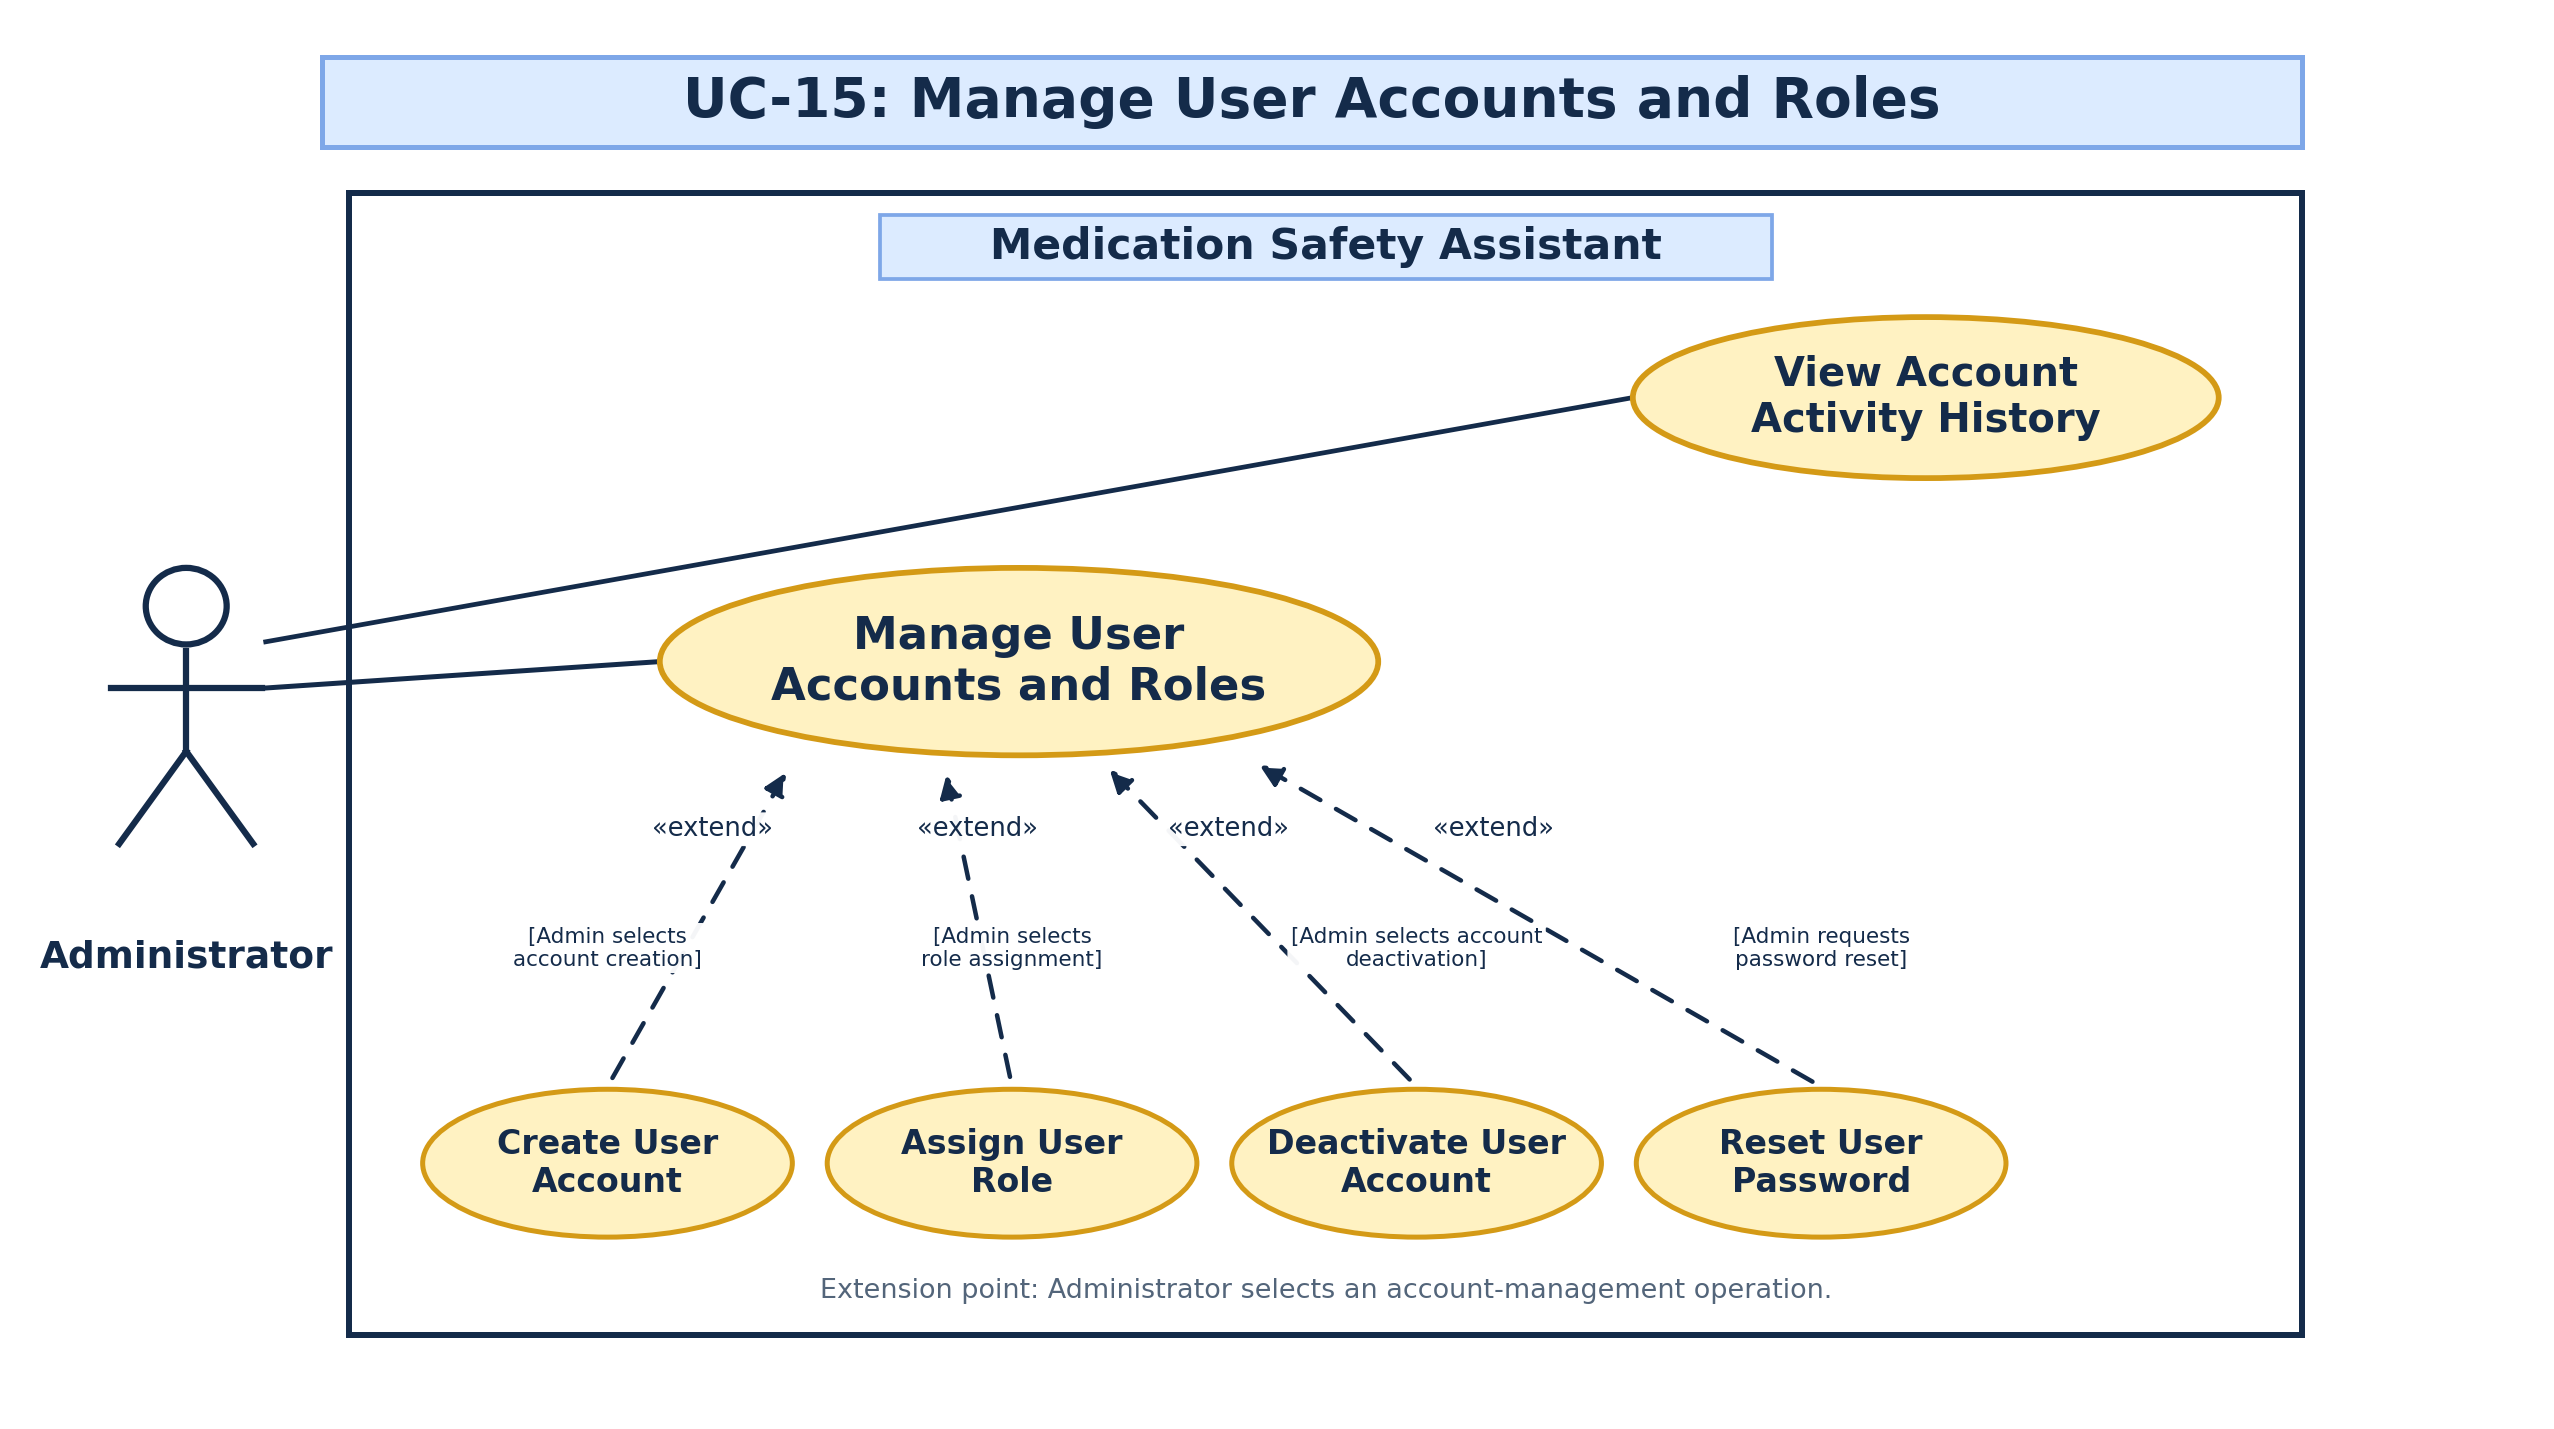
\includegraphics[width=0.91\textwidth,height=0.245\textheight,keepaspectratio]{images/UC-15.png}
    \caption{UC-15: Detailed use-case model.}
    \label{fig:uc-15}
\end{figure}
\begin{longtable}{|p{0.20\textwidth}|p{0.70\textwidth}|}
\hline
\textbf{Use case Name} & UC-15: Manage User Accounts and Roles \\ \hline
\textbf{Brief description} &
The Administrator creates or updates accounts and assigns permitted roles under the system access policy. \\ \hline
\textbf{Actors} & Administrator \\ \hline
\textbf{Basic Flow} &
1. The Administrator opens Manage User Accounts and Roles.\par
2. The system displays the account list, account status, and permitted role options.\par
3. The Administrator selects an account-management operation and provides the required details.\par
4. The system validates the request against account and role-based access control (RBAC) rules.\par
5. The system displays the proposed change, and the Administrator confirms it.\par
6. The system applies the authorized change and records the responsible Administrator and time.\par
7. The Administrator may view the account activity history.
\\ \hline
\textbf{Alternative Flows} &
\textbf{A1. Administrator creates a user account (step 3)}\par
The Administrator selects Create User Account and enters the required details. Continue to step 4.\par\smallskip
\textbf{A2. Administrator assigns a user role (step 3)}\par
The Administrator selects Assign User Role, chooses an account, and selects a permitted role. Continue to step 4.\par\smallskip
\UCchange{\textbf{A3. Administrator deactivates a user account (step 3)}}\par
\UCchange{The Administrator selects Deactivate User Account and chooses the account. The system checks whether deactivation is permitted (step 4). Only after confirmation (step 5) does the system deactivate access and save the activity record (step 6). Existing account records are retained.}\par\smallskip
\textbf{A4. Administrator resets a user password (step 3)}\par
The Administrator selects Reset User Password and chooses an account. The system prepares the authorized reset process. Continue to step 4.\par\smallskip
\textbf{A5. Request is invalid or not permitted (step 4)}\par
The system rejects the request without making changes or granting unauthorized permissions. The Administrator may correct the request.\par\smallskip
\textbf{A6. Administrator cancels or saving fails (steps 5--6)}\par
The previous account and role settings remain unchanged. The system reports the error when relevant.
\\ \hline
\textbf{Pre-conditions} &
The Administrator is signed in with account and role-management permission. \\ \hline
\textbf{Post-conditions} &
\textbf{Success:} The authorized account or role change is stored with an activity record.\par
\textbf{Failure:} No unconfirmed, invalid, or unauthorized change is applied.
\\ \hline
\end{longtable}
% ============================================================
% 09. TECHNICAL SUPPORT
% ============================================================
% UC-16 - Report Technical Issue
\clearpage
\subsection{Use-case: Report Technical Issue}
\label{uc:uc-16}
\InlineUCModel{16}
\begin{longtable}{|p{0.20\textwidth}|p{0.71\textwidth}|}
\hline
\endfirsthead
\multicolumn{2}{l}{\textbf{UC-16: Specification (continued)}}\\\\
\hline
\endhead
\textbf{Use case Name} &
\textcolor{blue}{UC-16: Report Technical Issue}
\\ \hline
\textbf{Brief description} &
A registered user reports a technical problem and receives a support ticket status.
\\ \hline
\textbf{Actors} &
\textcolor{blue}{Registered User (all registered roles)}
\\ \hline
\textbf{Basic Flow} &
1. The user opens Report Technical Issue.\par
2. The system shows the required issue fields and optional diagnostic details.\par
3. The user describes the problem and reviews any attached information.\par
\textcolor{blue}{4. The system displays the report details through Review Issue Details and Attachments.}\par
5. The user submits the report.\par
\textcolor{blue}{6. The system validates the required information and attachment rules.}\par
\textcolor{blue}{7. The system saves the ticket and displays its identifier and initial status only after successful creation.}
\\ \hline
\textbf{Alternative Flows} &
\textbf{A1. Required information is missing (step 6)}\par
1. The system highlights the missing information.\par
2. Return to step 3 for correction.
\\ \hline
\textbf{Alternative Flows} &
\textbf{A2. Attachment contains unnecessary patient information (step 3)}\par
1. The system requests removal or masking of the private data before submission.\par
2. Return to step 3.
\\ \hline
\textbf{Alternative Flows} &
\textbf{A3. User cancels or ticket creation fails (steps 5--7)}\par
1. No successful ticket submission is reported.\par
2. The user may retry after an error or end the use case.
\\ \hline
\textbf{Pre-conditions} &
The user is signed in and can open the technical support feature.
\\ \hline
\textbf{Post-conditions} &
\textbf{Success:} A support ticket is stored and its identifier and initial status are displayed without unnecessary patient data.\par
\textbf{Failure:} No ticket is created.
\\ \hline
\end{longtable}
% UC-17 - Handle Technical Support Request
\clearpage
\subsection{Use-case: Handle Technical Support Request}
\label{uc:uc-17}
\InlineUCModel{17}
\begin{longtable}{|p{0.20\textwidth}|p{0.71\textwidth}|}
\hline
\endfirsthead
\multicolumn{2}{l}{\textbf{UC-17: Specification (continued)}}\\\\
\hline
\endhead
\textbf{Use case Name} &
\textcolor{blue}{UC-17: Handle Technical Support Request}
\\ \hline
\textbf{Brief description} &
Technical Support investigates a permitted ticket, records progress, and provides an outcome when available.
\\ \hline
\textbf{Actors} & Technical Support \\ \hline
\textbf{Basic Flow} &
\textcolor{blue}{1. Support staff opens View Assigned Support Tickets and selects a ticket.}\par
2. The system shows the issue description, status, and allowed technical details.\par
3. Support staff investigates the issue and records relevant notes.\par
4. Support staff records a resolution or updates the ticket status.\par
\textcolor{blue}{5. The system saves the action, time, and responsible account and displays the updated ticket status to the reporting user.}
\\ \hline
\textbf{Alternative Flows} &
\textbf{A1. More information is required (step 3)}\par
1. Support staff requests only necessary technical details through Request Additional Technical Information.\par
2. The system records the request and marks the ticket Pending User Response.\par
3. The reporting user may provide additional information through the same ticket.\par
4. The system records the reply and returns the ticket to the support queue for continued handling.
\\ \hline
\textbf{Alternative Flows} &
\textbf{A2. The issue is not resolved (step 4)}\par
1. Support staff records progress and keeps the ticket Open or In Progress.\par
2. Continue to step 5.
\\ \hline
\textbf{Alternative Flows} &
\textbf{A3. Unauthorized patient data is present (step 2)}\par
1. The system restricts access to medical content.\par
2. Support staff works with permitted technical details only.
\\ \hline
\textbf{Alternative Flows} &
\textbf{A4. Access is denied or saving fails (steps 1 or 5)}\par
1. The system denies the action or reports the error.\par
2. No unsupported resolution is recorded.
\\ \hline
\textbf{Pre-conditions} &
Support staff is signed in and permitted to access the selected support ticket.
\\ \hline
\textbf{Post-conditions} &
\textbf{Success:} The ticket status and troubleshooting history are saved; the reporting user can view the updated status.\par
\textbf{Failure:} No unsupported ticket update or patient-data access occurs.
\\ \hline
\end{longtable}
% ============================================================
% 10. PATIENT HEALTH PROFILE
% ============================================================
% ==================== UC-18 ====================
% Source of truth: UC-18 diagram, including all six child use cases.
\subsection{Use-case: Manage Patient Health Profile}
\label{uc:uc-18}
\begin{figure}[H]
    \centering
    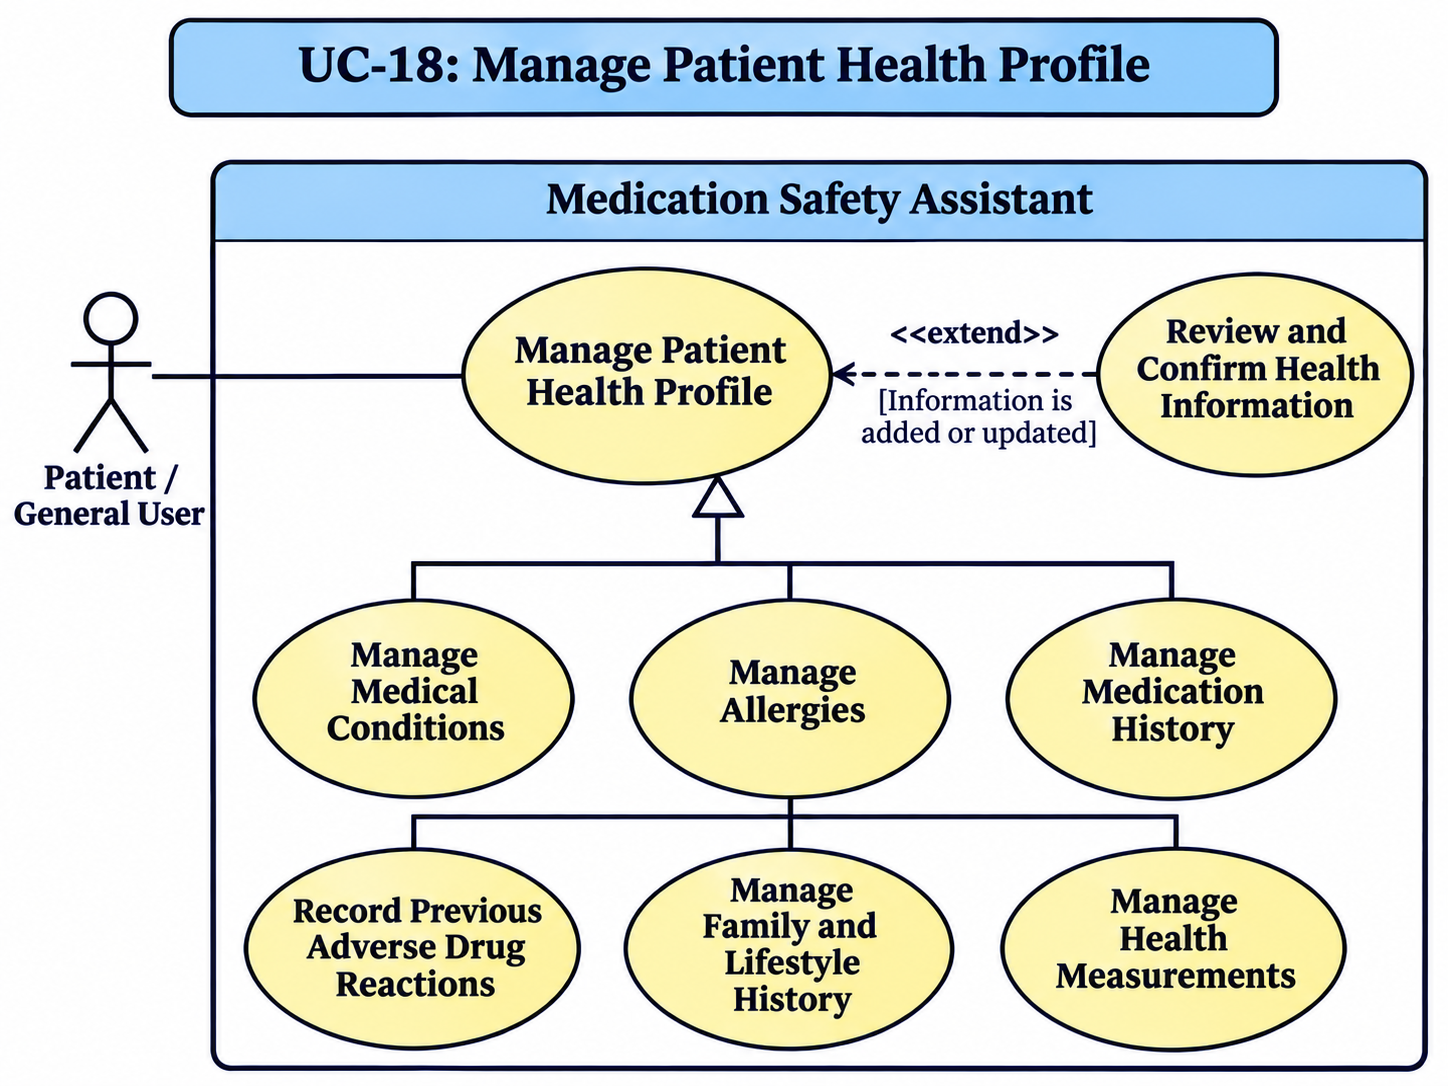
\includegraphics[width=0.91\textwidth,height=0.245\textheight,keepaspectratio]{images/UC-18.png}
    \caption{UC-18: Detailed use-case model.}
    \label{fig:uc-18}
\end{figure}
\begin{longtable}{|p{0.20\textwidth}|p{0.70\textwidth}|}
\hline
\textbf{Use case Name} & UC-18: Manage Patient Health Profile \\ \hline
\textbf{Brief description} &
\UCchange{The patient views and manages medical conditions, allergies, medication history, previous adverse drug reactions (ADRs), family and lifestyle history, and health measurements.} \\ \hline
\textbf{Actors} & Patient / General User \\ \hline
\textbf{Basic Flow} &
\UCchange{1. The patient opens Manage Patient Health Profile.}\par
\UCchange{2. The system shows medical conditions, allergies, medication history, previous ADRs, family/lifestyle history, and health measurements.}\par
\UCchange{3. The patient selects a category to view, add, or update an entry.}\par
\UCchange{4. For an addition or update, the patient enters the details, available source, and relevant status (e.g., current or discontinued medication).}\par
\UCchange{5. The system validates the details; the patient reviews and explicitly confirms the change (Review and Confirm Health Information).}\par
\UCchange{6. The system saves the confirmed information with its source, status, and update time.}
\\ \hline
\textbf{Alternative Flows} &
\UCchange{\textbf{A1. View only (step 3)}}\par
\UCchange{The system shows the selected entry. No confirmation or change is needed.}\par\smallskip
\UCchange{\textbf{A2. Missing or invalid details (steps 4--5)}}\par
\UCchange{The system highlights the issue. The patient may correct it and return to step 4.}\par\smallskip
\UCchange{\textbf{A3. Uncertain information or source (steps 4--5)}}\par
\UCchange{The system marks the limitation as patient-reported or uncertain. The patient may confirm it, but it is not clinically verified.}\par\smallskip
\UCchange{\textbf{A4. Patient cancels (step 5)}}\par
\UCchange{No proposed change is applied.}\par\smallskip
\UCchange{\textbf{A5. Saving fails (step 6)}}\par
\UCchange{The system reports the error and retains previously saved information.}
\\ \hline
\textbf{Pre-conditions} &
The patient is signed in and can access their own health profile. \\ \hline
\textbf{Post-conditions} &
\textbf{Success:} \UCchange{The patient views permitted information or saves a confirmed entry with provenance, status, and update time. Supported fields may inform UC-03 and UC-12; this is not clinical validation.}\par
\textbf{Failure:} Unconfirmed or failed updates are not applied.
\\ \hline
\end{longtable}
% ============================================================
% 11. PERSONAL MEDICATION CABINET
% ============================================================
% UC-19 - Manage Personal Medication Cabinet
\clearpage
\subsection{Use-case: Manage Personal Medication Cabinet}
\label{uc:uc-19}
\InlineUCModel{19}
\begin{longtable}{|p{0.20\textwidth}|p{0.71\textwidth}|}
\hline
\textbf{Use case Name} &
\textcolor{blue}{UC-19: Manage Personal Medication Cabinet}
\\ \hline
\textbf{Brief description} &
\textcolor{blue}{The patient manages a personal collection of medication records, including medication details and usage status. This use case is reserved for future development.}
\\ \hline
\textbf{Actors} &
Patient / General User
\\ \hline
\textbf{Basic Flow} &
\textcolor{blue}{1. The patient opens Manage Personal Medication Cabinet.}\par
\textcolor{blue}{2. The system displays the medications saved in the cabinet.}\par
\textcolor{blue}{3. The patient selects an operation: add a medication, view its details, update its information, update its usage status, or view expired and expiring medications.}\par
\textcolor{blue}{4. The system displays the relevant information or input fields.}\par
\textcolor{blue}{5. The patient confirms the requested changes.}\par
\textcolor{blue}{6. The system validates and saves the changes, then displays the updated information.}
\\ \hline
\textbf{Alternative Flows} &
\textcolor{blue}{A1. Required information is missing or invalid (step 5)}\par
\textcolor{blue}{1. The system highlights the missing or invalid information.}\par
\textcolor{blue}{2. The patient corrects the information and retries.}
\\ \hline
\textbf{Pre-conditions} &
\textcolor{blue}{The patient is signed in and can access the personal medication cabinet.}
\\ \hline
\textbf{Post-conditions} &
\textcolor{blue}{Success: Medication information and usage status are updated in the cabinet.}\par
\textcolor{blue}{Failure: No invalid or unconfirmed changes are saved.}
\\ \hline
\end{longtable}
\textcolor{blue}{\textbf{Scope note: This use case is reserved for future development and is not included in the current implementation scope.}}
% ============================================================
% 12. PERSONAL ACCOUNT
% ============================================================
% ==================== UC-20 ====================
\subsection{Use-case: Manage Personal Account}
\label{uc:uc-20}
\begin{figure}[H]
    \centering
    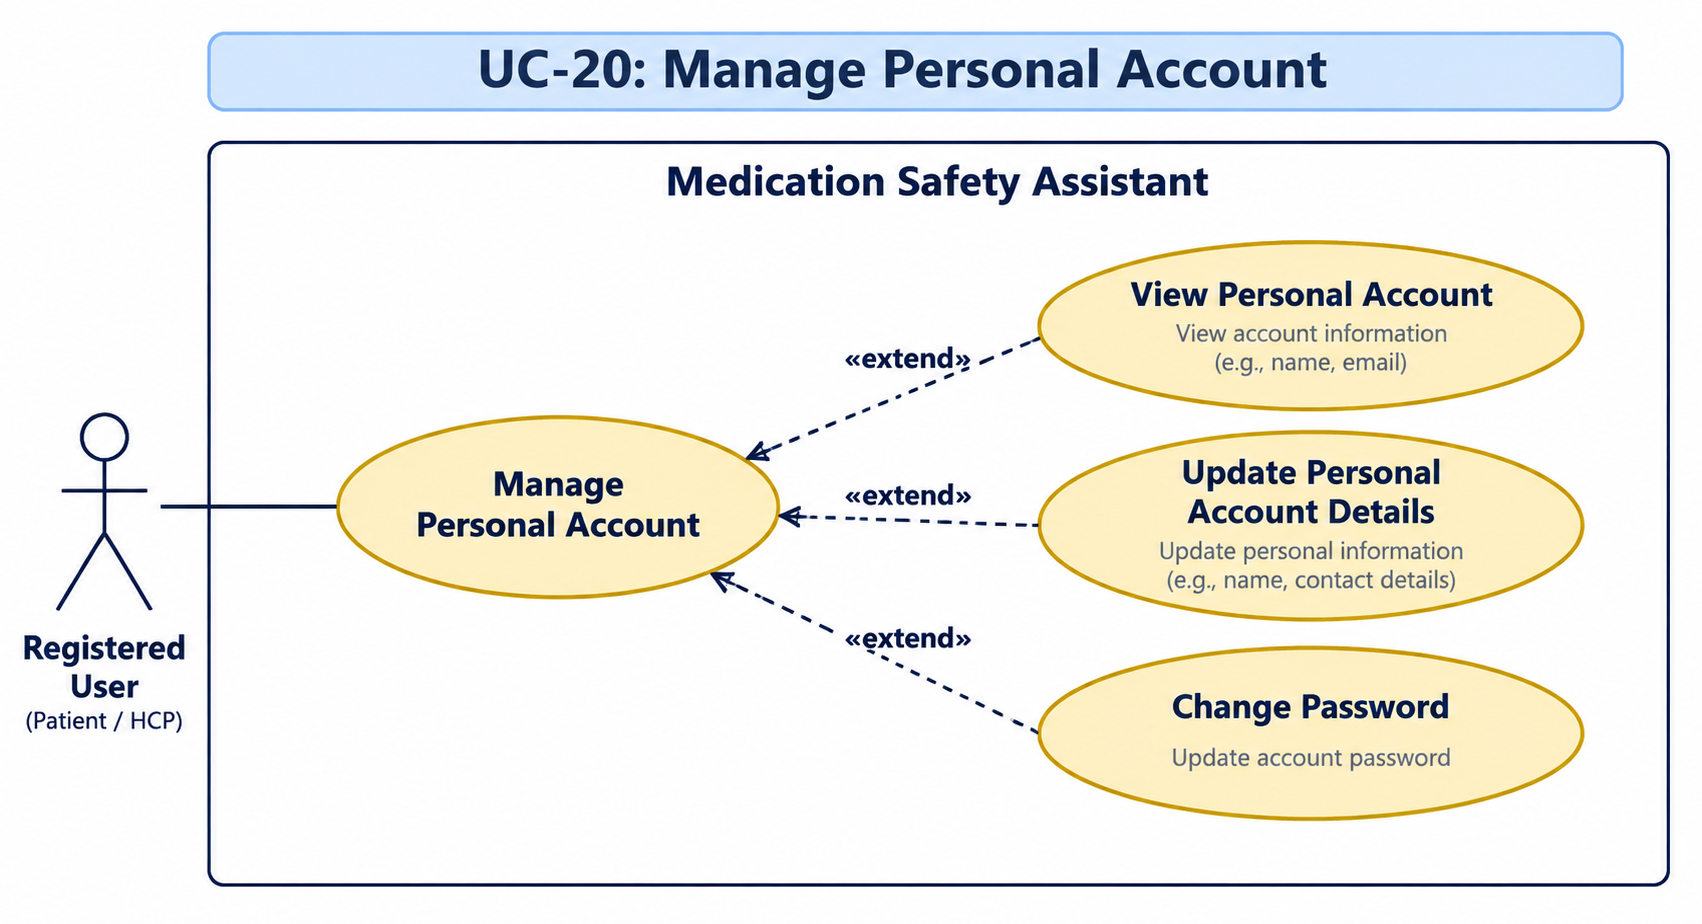
\includegraphics[width=0.91\textwidth,height=0.245\textheight,keepaspectratio]{images/UC-20.png}
    \caption{UC-20: Detailed use-case model.}
    \label{fig:uc-20}
\end{figure}
\begin{longtable}{|p{0.20\textwidth}|p{0.70\textwidth}|}
\hline
\textbf{Use case Name} & UC-20: Manage Personal Account \\ \hline
\textbf{Brief description} &
A registered user views or updates permitted personal account details or changes their password. \\ \hline
\textbf{Actors} &
\UCchange{All Registered Users (Patient / General User; Healthcare Professional (HCP); Administrator; Dataset Reviewer; Technical Support)} \\ \hline
\textbf{Basic Flow} &
1. The user opens Manage Personal Account.\par
2. The system displays the user's account information and permitted operations.\par
3. The user selects View Personal Account, Update Personal Account Details, or Change Password.\par
\UCchange{4. The system displays the selected information or input fields, and the user provides changes when needed.}\par
\UCchange{5. For an update, the system validates the request and saves it only after the user confirms the change.}\par
6. The system displays the result.
\\ \hline
\textbf{Alternative Flows} &
\textbf{A1. View personal account (step 3)}\par
The system displays the permitted account details. No account information is changed; continue to step 6.\par\smallskip
\textbf{A2. Update personal account details (steps 4--5)}\par
The user edits permitted details. The system validates them, requests confirmation, and saves an authorized change. Continue to step 6.\par\smallskip
\textbf{A3. Change password (steps 4--5)}\par
The user enters the current password, new password, and confirmation. The system verifies the current password, validates the new password, and updates it after confirmation. Continue to step 6.\par\smallskip
\textbf{A4. Information or password is invalid (step 5)}\par
The system displays an error without saving the change. The user may correct the input and retry.\par\smallskip
\UCchange{\textbf{A5. User cancels or saving fails (steps 4--5)}}\par
\UCchange{The system keeps the existing account information and password unchanged and reports any saving error.}
\\ \hline
\textbf{Pre-conditions} &
The user is signed in and has permission to access their own account. \\ \hline
\textbf{Post-conditions} &
\UCchange{\textbf{Success:} The requested account details are viewed or an authorized update is saved. Assigned roles and permissions remain unchanged.}\par
\textbf{Failure:} No invalid, unconfirmed, or unauthorized account change is saved.
\\ \hline
\end{longtable}